\documentclass[12pt]{article}
\usepackage[portuguese]{babel}
\usepackage[utf8]{inputenc}
\usepackage[usenames,dvipsnames]{color}
\usepackage{setspace}
\usepackage{amsmath}
\usepackage{amsfonts}
\usepackage{amssymb}
\usepackage{mathtools}
\usepackage[top=3cm, bottom=2cm, left=3cm, right=2cm]{geometry}
\usepackage{tikz}
\usepackage{indentfirst}
\usepackage{textcomp}
\title{Relatorio IC}

% packages added by Marcelo
%
\usepackage{lscape}    % for landscape pages
\usepackage{hyperref}  % to allow hyperlinks
\usepackage{booktabs}  % nicer table borders
\usepackage{subfigure} % add subfigures

\graphicspath{{./figures/}} 

\definecolor{myblue}{RGB}{80,80,160}
\definecolor{mygreen}{RGB}{80,160,80}
\setstretch{1.5}

\begin{document}

% FAPESP demands the usage of double spacing
%
\doublespacing

\begin{titlepage}
	\vfill 
	\begin{center}
        {\Large Relatório Científico Parcial -- Iniciação Científica\\
         \bigskip
         Processo FAPESP 2014/23564-0
        }
        
        \bigskip
    
  		{\LARGE Estudos de estruturas de dados eficientes para abordar o\\
    	\bigskip
    	problema de otimização U-curve}

        \bigskip
  		\bigskip
  		{\Large {\bf Beneficiário:} \href{mailto:gustavo.estrela.matos@usp.br}{Gustavo Estrela de Matos}\\ 
        
  		{\bf Responsável:} \href{mailto:marcelo.reis@butantan.gov.br}{Marcelo da Silva Reis}\\

        \bigskip
        \bigskip
        \bigskip
  		\bigskip
        \bigskip
  		\bigskip
        \bigskip
Relatório referente aos trabalhos desenvolvidos entre 1 de janeiro e 10 de junho de 2015

        \bigskip
        \bigskip
        \bigskip
  		\bigskip
        \bigskip
  		\bigskip
        \bigskip

Laboratório Especial de Toxinologia Aplicada, Instituto Butantan\\
        \bigskip
  		São Paulo, \today\\
  		}

  		\bigskip
        \bigskip

       

\end{center}
\end{titlepage}


\tableofcontents

\pagebreak



\section{Resumo do Projeto Proposto} \label{sec:resumo} % até 2 páginas


%% O texto desta seção poderá ser este: basicamente é o resumo do projeto, com algumas poucas atualizações para refletir
%% o estágio atual do projeto


O problema de otimização U-curve pode ser utilizado para modelar problemas em diversas áreas; por exemplo, o problema de seleção de características em Reconhecimento de Padrões. Um algoritmo ótimo para abordar o problema U-curve é o U-Curve-Search ({\tt UCS}). Esse algoritmo alcançou resultados promissores na solução desse problema, pois computa poucas vezes a função custo; porém, em sua atual implementação, {\tt UCS} tem problemas de escalabilidade, o que se deve em grande medida à utilização de listas duplamente encadeadas para armazenar o controle do espaço de busca já percorrido pelo algoritmo. Dessa forma, propomos neste projeto de Iniciação Científica a investigação do uso de diagramas de decisão binária reduzidos e ordenados (ROBDDs) como solução de estrutura de dados para controlar o espaço de busca já percorrido pelo algoritmo {\tt UCS}. Utilizamos ROBDDs para desenvolver o algoritmo {\tt UCSR}, uma nova versão do {\tt UCS} que foi implementada e testada utilizando o arcabouço featsel. Realizamos testes com instâncias artificiais e, em breve, utilizaremos também dados de problemas reais, tais como a etapa de seleção de características durante o desenho de W-operadores. Resultados iniciais mostraram que {\tt UCSR} é mais eficiente do que {\tt UCS} do ponto de vista de consumo de tempo computacional, o que sugere que o novo algoritmo é mais competitivo para resolver problemas práticos que possam ser descritos como um problema de otimização U-curve.


\pagebreak

\section{Atividades Realizadas} \label{sec:atividades}  % até 10 páginas
%% ------------- TODO -------------
%%
%Num último parágrafo, você apresentará ao leitor deste relatório o que virá ao longo do restante desta seção. "Na  seção~\ref{sec:atividades:ROBDD}, descreveremos a implementação do ROBDD no arcabouço...
%%
%% ------------- TODO -------------

%% O texto nesta seção precisará ser modificado; eu coloquei apenas um rascunho do que, em linhas gerais, entendo
%% que precisará entrar nesta seção.

%
% A considerar: talvez seja interessante, antes de relembrar propriedades de interesse do UCS, uma breve recapitulação do que 
% seria o problema U-curve (em 1 parágrafo).
%

As seções a seguir apresentam as atividades realizadas nos seis primeiros meses de trabalho no projeto. Na seção \ref{sec:atividades:estudo} apresentamos conceitos fundamentais que foram estudados no início das atividades para a realização do projet. Na seção \ref{sec:atividades:ROBDD} mostramos as principais características da estrutura de dados ROBDD implementada no arcabouço {\tt featsel}. Na seção \ref{sec:atividades:DFS} descrevemos as simplificações da busca em profundidade do {\tt UCS} implementadas no {\tt UCSR3, UCSR4, UCSR5} e {\tt UCSR6}. Na seção \ref{sec:atividades:ajuste} explicamos o ajuste feito, entre tempo de execução e número de chamadas da função custo, implementados no algoritmo {\tt UCSR6}. Na seção \ref{sec:atividades:resultados} apresentamos os resultados dos algoritmos implementados, comparando também com {\tt UCS} e com Exhaustive Search ({\tt ES}), uma implementação de busca exaustiva do espaço de busca.


%%%Iniciamos esta seção relembrando alguns fatos: 
\subsection{Estudo do algoritmo {\tt UCS} e de ROBDDs}\label{sec:atividades:estudo}
Para criar novos algoritmos para solucionar o problema U-Curve, baseamo-nos na dinâmica do algoritmo {\tt U-Curve-Search} ({\tt UCS}), conforme apresentado em Reis~\cite{msreis thesis}. Este algoritmo estrutura o espaço de busca como um recitulado Booleano e, através de uma busca em profundidade e com o auxilio de restrições ao espaço de busca, determina uma solução ótima para o problema. 

No algoritmo {\tt UCS} as restrições do espaço de busca são representadas por duas listas de restrições: inferior e superior. Essas listas armazenam vários elementos do espaço de busca, e cada elemento representa um intervalo que está restrito (i.e., um intervalo de elementos que foram removidos do espaço de busca corrente). Se um elemento $X$ pertence a lista inferior (no caso dual, superior), temos que o intervalo $[\emptyset, X]$ ($[X, S]$) não está no espaço de busca. Estas listas foram implementadas com o uso de listas duplamente encadeadas, e para consultar se um elemento está no espaço de busca é necessário verificar se algum dos intervalos das listas cobre (i.e. contém) este elemento. Mais informações sobre o {\tt UCS} podem ser encontradas em Reis ~\cite{msreis thesis}, \cite{ucs paper}.

Visando melhorar o controle de espaço de busca, desenvolvemos novos algoritmos para o problema U-Curve utilizando diagramas de decisão binária ordenadas e reduzidas ({\em Reduced Ordered Binary Decision Diagrams} -- ROBDDs~\cite{bryant}). Esses diagramas representam, através de árvores, funções Booleanas $f:B^{n} \rightarrow B$ ($B = \{0, 1\}$); portanto, podemos controlar o espaço de busca utilizando um ROBDD tal que $f(X)$ vale 1 se $X$ está fora do espaço de busca e 0 caso contrário. Além disso, consultar se um elemento pertence ao espaço de busca em um ROBDD é linear em relação a $n$ (cardinalidade do conjunto de características) como pode ser visto na figura \ref{fig:ROBDDs}.

\begin{figure}[!ht]
  \centering 
    \subfigure[] {\scalebox{0.75}{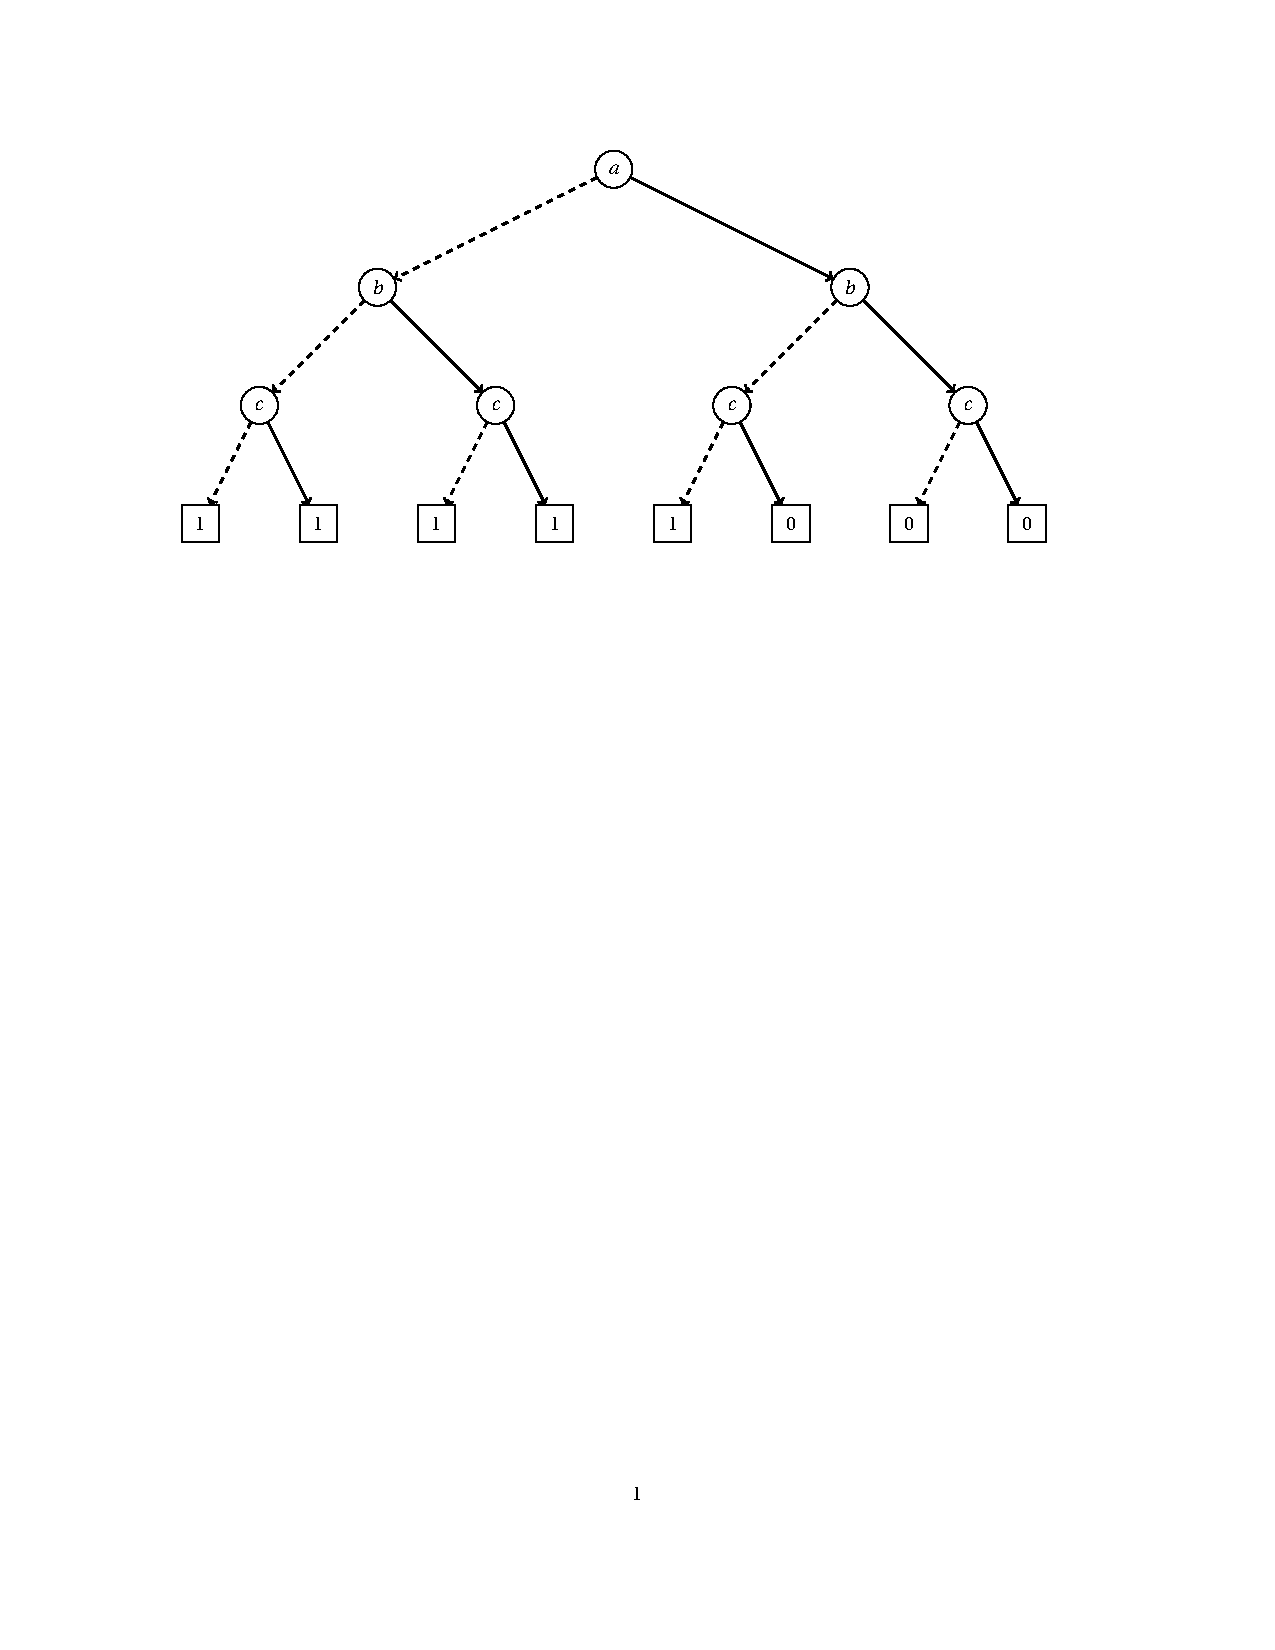
\includegraphics[trim=2cm 17.5cm 2cm 2cm, clip=true]{Binary_tree_3.pdf}}  \label{fig:ROBDDs:A}}  
  \begin{tabular}{c c}
    \subfigure[] {\scalebox{0.75}{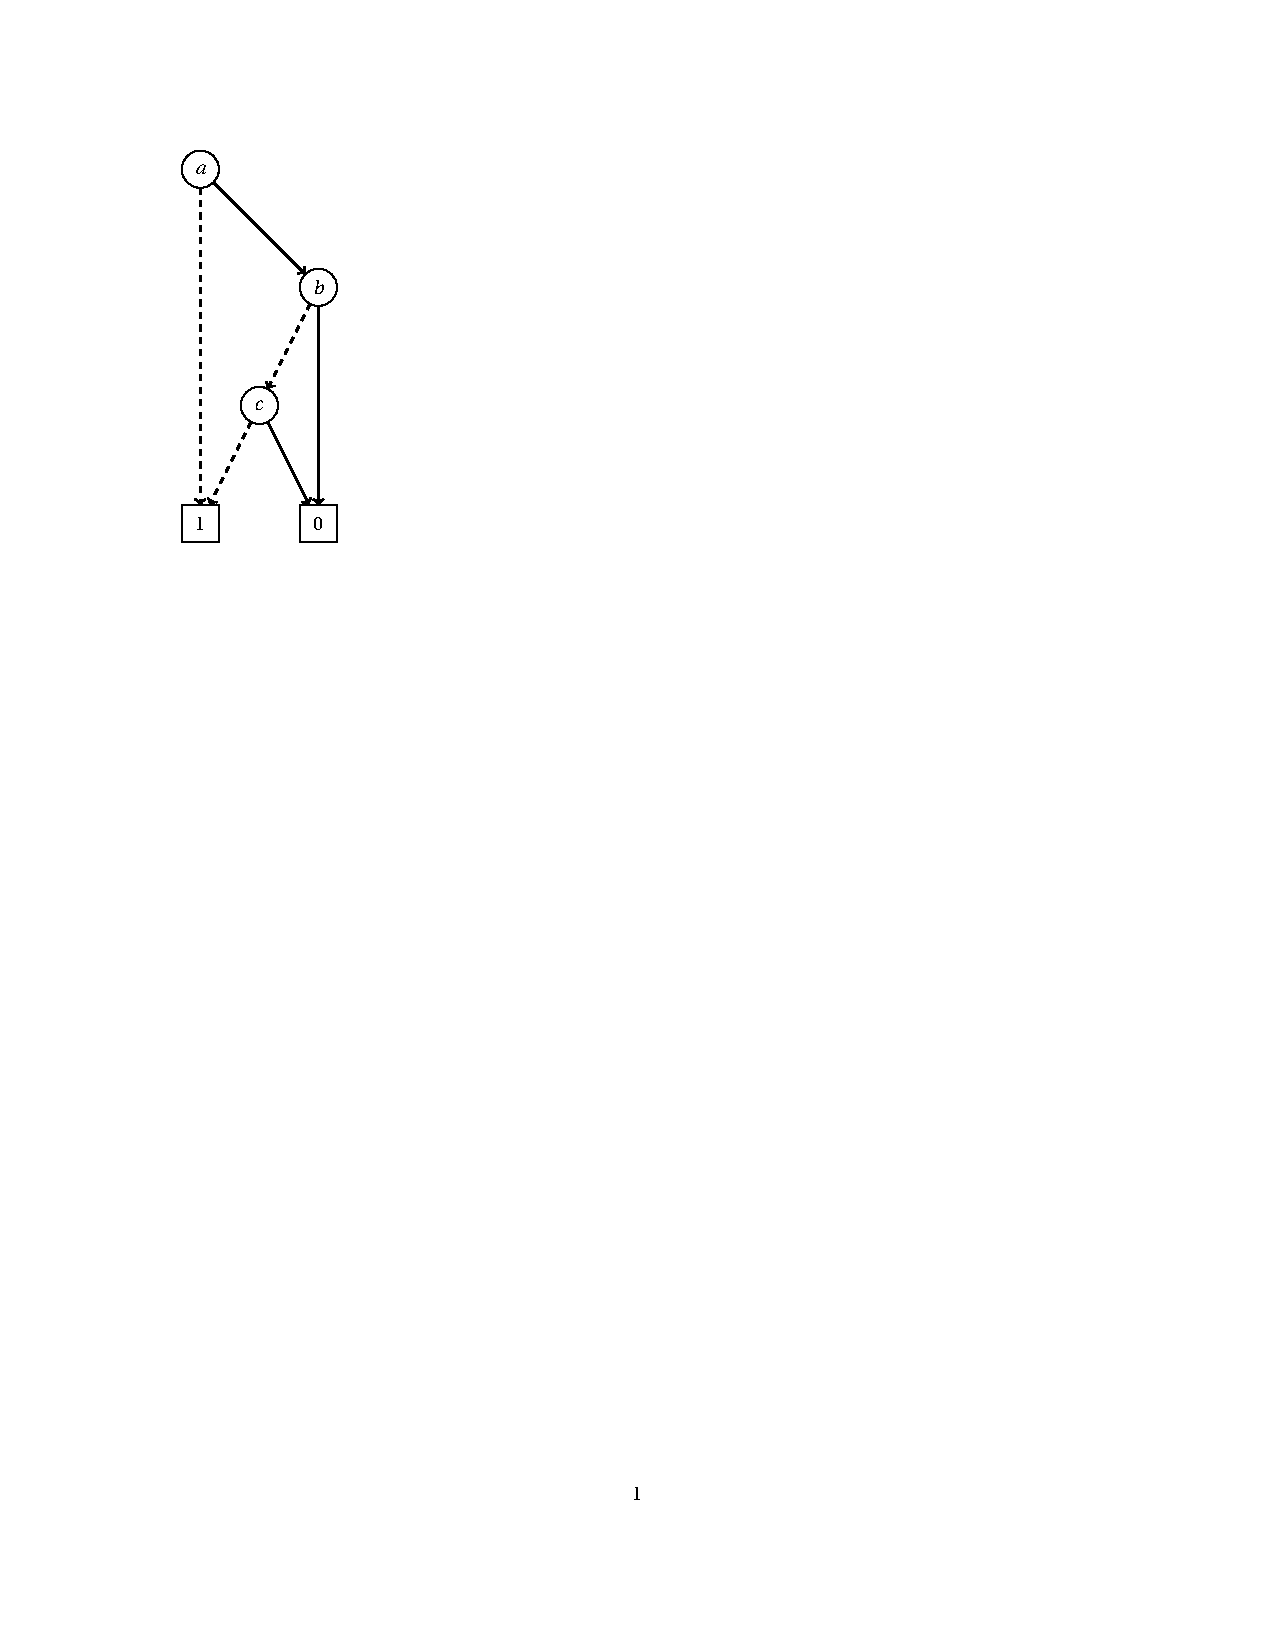
\includegraphics[trim=0cm 17.5cm 12.2cm 2cm, clip=true]{ROBDD_good.pdf}}  \label{fig:ROBDDs:B}}  
  &
        \subfigure[] {\scalebox{0.75}{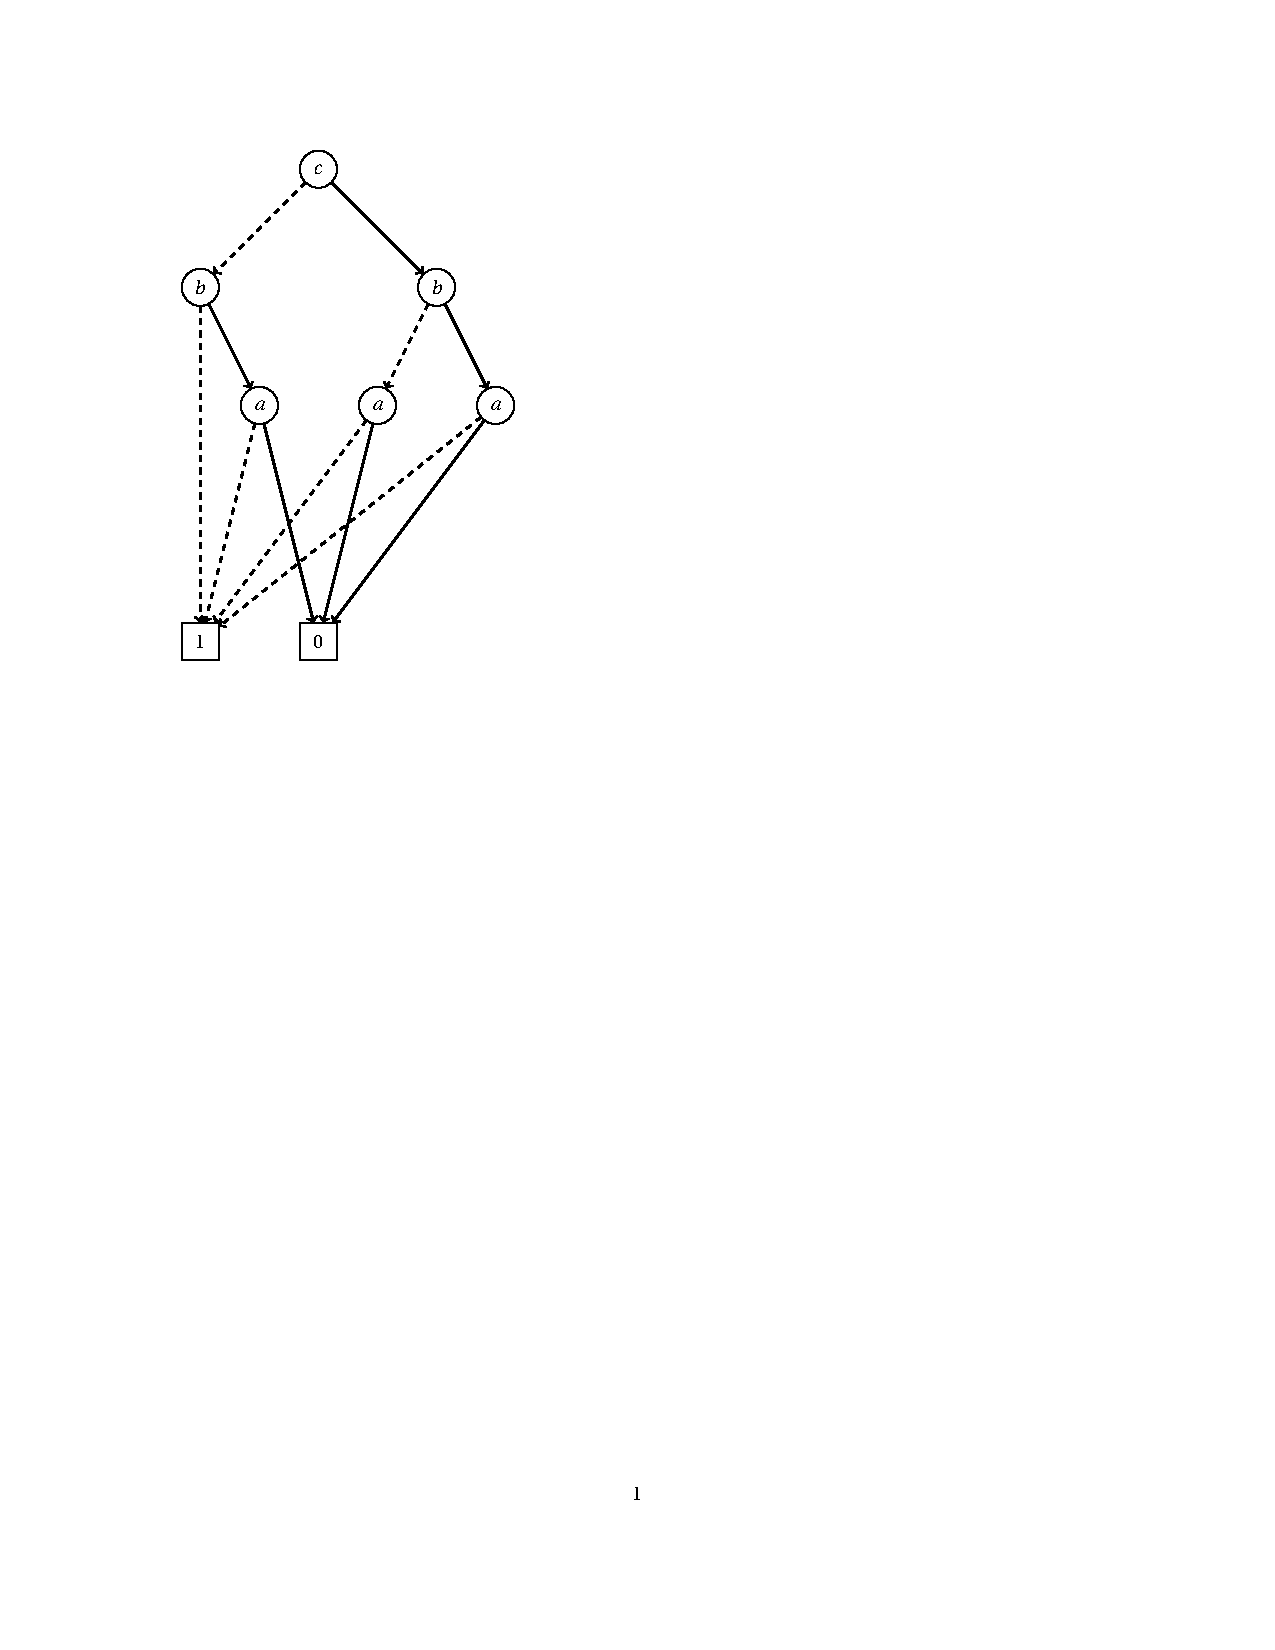
\includegraphics[trim=1cm 15.5cm 12cm 2cm, clip=true]{ROBDD_bad.pdf}}  \label{fig:ROBDDs:C}}  
  \end{tabular}
  \caption{exemplo do uso de ROBDDs para representar o espaço de busca corrente durante a execução do algoritmo {\tt UCS}. Figura~\ref{fig:ROBDDs:A}: árvore binária que representa um espaço de busca arbitrário; um arco sólido (pontilhado) representa que o elemento da ponta superior está (não está) presente no subconjunto considerado. Uma folha tem valor $1$ se um subconjunto está fora do espaço de busca corrente e $0$ caso contrário. Figura~\ref{fig:ROBDDs:B}: ROBDD obtido através da redução da árvore de decisão binária da figura~\ref{fig:ROBDDs:A}. Figura~\ref{fig:ROBDDs:C}: ROBDD obtido através da redução de uma árvore de decisão binária cuja raiz é o elemento $c$ ao invés de $a$; a redução dessa árvore produz um ROBDD com mais elementos do que o exibido na figura~\ref{fig:ROBDDs:B}.} 
  \label{fig:ROBDDs} 
\end{figure}

%\begin{itemize}
%
%	\item{i.} o algoritmo UCS original estrutura o espaço de busca como um reticulado  Booleano; 
%
%	\item{ii.} o gerenciamento do espaço de busca no UCS é feito através do armazenamento de pontas de intervalos do tipo $[\emptyset, X]$ ou %$[X, S]$, onde $X$ é uma ponta de intervalo; tais intervalos definem regiões que foram excluídas do espaço de busca corrente; 
%
%	\item{iii.} a consulta se um elemento $X$ pertence ao não ao espaço de busca é feita verificando se X é coberto por alguns dos intervalos %removidos do espaço de busca; a operacionalização da consulta faz uso de listas duplamente encadeadas.
%
%\end{itemize}
%
%Então informamos ao leitor que maiores detalhes do funcionamento de UCS podem ser obtidos em~\cite{msreis thesis} e \cite{ucs paper}. 
%Após isso, recapitulamos o que é um ROBDD, e como seria o gerenciamento do espaço de busca no reticulado Booleano utilizando ROBDDs; aqui você %poderia citar \cite{bryant} e \cite{brace}, e reaproveitar as figuras que estão no nosso projeto.


\subsection{Implementação de ROBDDs no arcabouço {\tt featsel} } \label{sec:atividades:ROBDD}
A implementação do ROBDD foi feita utilizando o {\tt featsel}, um arcabouço orientado a objetos desenvolvido em C++ que permite, entre outras funcionalidades, implementar algoritmos que utilizam elementos de um reticulado Booleano. A classe ROBDD possui métodos que permitem mudar o espaço de busca representado e é definida pela raíz da árvore, um objeto da classe Vértice.

A classe Vértice possui uma estrutura que guarda um elemento do reticulado Booleano, para nós internos da árvore, ou um valor Booleano, para as folhas da árvore. Os elementos dos vértices são instâncias da classe ElementSubset do arcabouço {\tt featsel}; os detalhes de implementação desta última podem ser encontradas em Reis ~\cite{msreis thesis}. Além disso, os vértices possuem duas referências para outros vértices permitindo a criação da árvore em si.

Para mudar a função que representa o espaço de busca atual no ROBDD, criamos o método \emph{add\_interval}, que recebe como parametro um elemento $X$ e uma variável indicadora que decide qual intervalo será restrito, $[\emptyset, X]$ ou $[X, S]$. Neste método cria-se uma árvore temporária que representa o intervalo adicionado e une-se a ela o ROBDD original. Para realizar a união entre a árvore que descreve o espaço de busca corrente e a árvore temporária, implementamos o algoritmo proposto por Bryant e Randal~\cite{bryant}.

A partir destas classes e também de outras existentes no arcabouço, criamos vários algoritmos que utilizam ROBDDs para gerenciar o espaço de busca corrente: por exemplo, o {\tt UCSR2}, que possui a mesma dinâmica que o algoritmo {\tt UCS}, mas utiliza um ROBDD ao invés de duas listas de restrições. Também criamos os algoritmos {\tt UCSR3, UCSR4, UCSR5} e {\tt UCSR6} que, além do uso de ROBDDs, têm em comum o fato de utilizarem uma dinâmica simplificada da busca em produndidade, que será explicada a seguir.
%Nesta seção, devemos iniciar apresentando as principais características do arcabouço featsel. Para maiores detalhes sobre esse arcabouço, você poderá recomendar ao leitor ler~\cite{msreis thesis}.
%Na sequência, você apresentará a classe ROBDD que foi implementada nesse ambiente, suas principais propriedades. Se achar apropriado, você também pode apresentar o diagrama de classes da implementação de ROBDDs.
%Por fim, você dirá que novas versões do algoritmo foram criadas: uma com ROBDD no lugar de duas listas (UCSR2) e outra sem redução do diagrama (UCSR3). Comentar brevemente sobre o desempenho de cada um desses dois algoritmos e dizer qu resultados experimentais se encontram na tabela~\ref{tab:comparison}.


\subsection{Simplificação da busca em profundidade ({\em DFS}) feita pelo algoritmo original} \label{sec:atividades:DFS}

O algoritmo {\tt UCS} possui uma busca em profundidade complexa que depende do uso de estruturas de dados para grafos. Essas estruturas armazenam elementos já visitados do espaço de busca mas que ainda não podem definir a ponta de um intervalo a ser removido do espaço de busca, sob o risco de perder o mínimo global. Tal risco ocorre em situações onde ocorrem empates no custo de dois elementos adjacentes entre si na cadeia do reticulado~\cite{msreis thesis}. Todavia, o uso desse grafo resulta num consumo alto tanto de memória quanto de processamento. 


Todavia, em instâncias de problemas de interesse prático que podem ser modelados como um problema U-curve, empates de custo entre elementos adjacentes é uma situação que raramente ocorre. Ademais, nas instâncias ``difíceis" que utilizamos para realizar os testes, para cada cadeia do reticulado, é possível a ocorrência de no máximo um empate entre elementos adjacentes. Chamamos essa situação de ``empate simples". Por conta disso, passamos a inverstigar simplificações na busca em profundidade.

A primeira solução nova nos levou ao algoritmo {\tt UCSR3}, que possui uma dinâmica bem parecida com a do UCS, porém sem guardar elementos visitados em um grafo, estratégia útilizada no {\tt UCS} para determinar a sequência da busca em casos de empates. Neste novo algoritmo, no caso em que dois elementos $X \subset Y$ são adjacentes e possuem o mesmo custo, olhamos para um elemento $Z \subset X$ e se seu custo foi maior (menor) que o de $X$, restringimos o intervalo $[\emptyset, X]$ ($[X, S]$). O caso em que haja empate de custo entre $Z$ e $X$ (i.e., empate entre três ou mais elementos adjacentes dois a dois) não é tratado neste algoritmo.

Ainda com a hipótese de que há no máximo empates simples, elaboramos uma outra dinâmica, presente nos algoritmos {\tt UCSR4, UCSR5} e {\tt UCSR6}. Nesta nova dinâmica fazemos um passeio pelo espaço de busca seguindo as seguintes regras, partindo de um elemento $X$ do espaço de busca, com $Y$ adjacente a $X$:
\begin{itemize}
\item[i.] Se $Y$ é adjacente superior (inferior) e tem custo menor que $X$, restringimos o intervalo $[\emptyset, X]$ ($[X, S]$) e passamos a avaliar $Y$;
\item[ii.] Se $Y$ é adjacente superior (inferior) e tem custo maior que $X$, podemos restringir, ou não, como será discutido na próxima sessão, o intervalo $[Y, S]$ ($[\emptyset, Y]$);
\item[iii.] Se $Y$ é adjacente superior (inferior) e tem custo igual a $X$ não fazemos nada;
\item[iv.] Paramos quando não houverem mais elementos adjacentes a $X$.
\end{itemize}

No algoritmo {\tt UCSR4}, dado um nó $X$ e o conjunto de características $S = \{x_1, x_2, ..., x_n\}$, o i-ésimo elemento adjacente a $X$ visitado será $Y_i$ tal que $(Y_i \cup X) \setminus (Y_i \cap X) = {x_i}$. Por exemplo, se $X = 00101$ então os vizinhos de $X$ visitados (assumindo que todos serão visitados) serão, na ordem: $10101$, $01101$, $00001$, $00111$ e $00100$. Note que, dependendo da composição de $X$, podemos visitar muitos elementos adjacentes superiores sem visitar nenhum elemento adjacente inferior, o que pode causar mais cálculos do que o necessário para visitar um elemento adjacente de menor custo.

Visando melhorar o percorrimento de elementos adjacentes, formulamos o {\tt UCSR5}, que percorre os elementos adjacentes intercalando as visitas entre vizinhos superiores e inferiores, enquanto possível. Por exemplo, se $X = 00100$, uma possível sequência de vizinhos visitados (assumindo que todos serão visitados) é, na ordem: $10100$, $00000$, $00110$, $01100$ e $00101$. Podemos ver na tabela \ref{tab:comparison:time}, essa mudança no percorrimento de vizinhos trouxe melhorias no tempo de execução em relação ao {\tt UCSR4}.


%Aqui você inicia constatando que a execução da busca em profundidade ({\em depth-first search -- DFS}) feita pelo algoritmo UCS original tinha um controle muito complicado e que provavelmente redundava em um grande gasto de tempo computacional. 
%A partir dessa hipótese, construímos duas novas versões do algoritmo com DFS simplificado, os UCSR4 e UCSR5. Explicar brevemente os princípios gerais de cada um deles.
% UCSR3 = UCSR2 sem grafo
% UCSR4 = simplificação, percorre vizinhos assim ->
% UCSR5 = percorre vizinho assim ^v^v
% UCSR6 = percorre vizinho assim ^v^v joga fora todos adjacentes e maiores

\subsection{Ajuste entre tempo de execução e número de chamadas da função custo} \label{sec:atividades:ajuste}

Como vimos na seção \ref{sec:atividades:DFS}, a nova dinâmica não especifica se devemos restringir um elemento $Y$ adjacente a $X$ e com custo maior. Se não restringirmos esse elemento corremos o risco de ter que recomputar seu custo, pois, diferentemente do {\tt UCS}, os algoritmos {\tt UCSR4}, {\tt UCSR5} e {\tt UCSR6} não possuem estrutura que guarda o custo dos elementos visitados. Porém, o elemento $Y$ pode estar contido em algum intervalo que será restrito em futuras iterações, tornando desnecessário restringir $Y$ logo no momento que o visitamos.

Portanto, temos um \emph{tradeoff} entre atualizações do ROBDD e cálculo de função de custo. Uma atualização nas restrições implica na construção de um ROBDD temporário, que representa o novo intervalo restrito, e sua união com o ROBDD que representa as novas restrições. Como visto em Randal e  Bryant \cite{bryant}, essa operação tem complexidade $O(|R_1| * |R_2|)$, em que $|R_1|$ e $|R_2|$ são as quantidades de nós das árvores que representam os ROBDDs atual e temporário, respectivamente. Por outro lado, não restringir um elemento de custo maior pode fazer com que calculemos o custo de um mesmo nó do reticulado mais de uma vez, o que, dependendo da função de custo, pode levar a um grande número de cálculos desnecessários.

Com o intuito de comparar as duas escolhas possíveis, desenvolvemos os algoritmos {\tt UCSR5}, que não restringe todo elemento adjacente com custo maior visitado, e o {\tt UCSR6}, que restringe esses elementos. Como podemos verificar na tabela \ref{tab:comparison:time} o algoritmo {\tt UCSR5} teve desempenho em tempo um pouco melhor do que o {\tt UCSR6}, que por sua vez teve menos cálculos da função custo, fato que podemos constatar na tabela~\ref{tab:comparison:costfunction}. 

%Nesta seção você apresenta a questão do {\em trade off} que surgiu na versão simplificada do DFS: entre tempo de execução e número de chamadas da função custo. É importante ressaltar que esse trade off, no fundo, diz respeito ao nível de recálculo que estamos permitindo para a função custo e também ao número de vezes que precisamos atualizar o espaço de busca corrente (e o que isso implica no ROBDD). Citar que um melhor ajuste que conseguimos foi com o algoritmo UCSR6.


%
%
\subsection{Resultados dos experimentos} \label{sec:atividades:resultados}
Para testar os algoritmos criados neste projeto, tendo como {\em benchmarking} os algoritmos {\tt UCS} original e {\tt ES}, utilizamos um programa em Perl que foi desenvolvido para esse fim. Nesse programa, para cada tamanho de $S$, diversas instâncias de problemas de tamanho $|S|$ foram geradas aleatóriamente a partir de reduções polinomiais do problema subset sum, que é NP-difícil \cite{msreis thesis}. Para cada instância e para cada algoritmo, o arcabouço {\tt featsel} era chamado, guardando ao final da execução o tempo computacional que foi exigido e o número de chamadas da função custo. Os resultados foram então agrupados por tamanho de instância e tiveram suas médias calculadas. Nas tabelas \ref{tab:comparison:time} e \ref{tab:comparison:costfunction} mostramos os resultados em termos de tempo e de número de chamadas da função custo, respectivamente..

%Você poderá abrir esta seção dizendo que todas as classes e algoritmos foram implementados utilizando o controle de versão git implementado no portal GitHub.

%Em seguida, explicar que todos os testes foram feitos utilizando instâncias "difíceis", geradas aleatoriamente a partir de reduções polinomiais do problema subset sum (um problema NP-difícil), conforme explicado em \cite{msreis thesis}. Para produzir as instâncias e rodar os algoritmos, foi utilizado um programa auxiliar escrito em Perl, que "embala" o arcabouço featsel.

%Nas tabelas X e Y, apresentamos os resultados dos testes. Para utilizar como {\em benchmarking} para os testes dos novos algoritmos, também rodamos os testes sobre o UCS original e também sobre uma busca exaustiva (ES).


%
% Coloquei aqui a tabela de resultados até $2^{19}$!
%
%
% TODO: quebre a tabela abaixo em 2 tabelas diferentes: uma para tempo e outra para número de chamadas da função custo.
% Se der, remova o landscape e volte a tabela para o layout normal da página.
%
%
% OBS: TIRAR UBB da tabela e deixar somente ES como benchmarking! Irá facilitar a nossa vida no relatório.
%
%

\begin{table}[ht] \begin{center} \begin{tabular}{@{}ccc ccc ccc ccc ccc ccc ccc ccc ccc cc@{}} \toprule
\multicolumn{2}{c}{Instância} & \multicolumn{7}{c}{Tempo (segundos)}\\
\cline{1-2} \cline{4-10} 
$|S|$ & $2^{|S|}$  &&  UCSR6 & UCSR5 & UCSR4 & UCSR3 & UCSR2 & UCS & ES    \\ \hline
 1 &       2 &&  0.00 & 0.00 & 0.00 & 0.00 & 0.00 & 0.00 & 0.00 & \\ 
 2 &       4 &&  0.00 & 0.00 & 0.00 & 0.00 & 0.00 & 0.00 & 0.00 & \\ 
 3 &       8 &&  0.00 & 0.00 & 0.00 & 0.00 & 0.00 & 0.00 & 0.00 & \\ 
 4 &      16 &&  0.01 & 0.01 & 0.01 & 0.01 & 0.01 & 0.01 & 0.00 & \\ 
 5 &      32 &&  0.01 & 0.01 & 0.01 & 0.01 & 0.01 & 0.01 & 0.01 & \\ 
 6 &      64 &&  0.01 & 0.01 & 0.01 & 0.01 & 0.01 & 0.01 & 0.01 & \\ 
 7 &     128 &&  0.01 & 0.01 & 0.01 & 0.01 & 0.02 & 0.02 & 0.01 & \\ 
 8 &     256 &&  0.02 & 0.02 & 0.02 & 0.02 & 0.03 & 0.03 & 0.02 & \\ 
 9 &     512 &&  0.04 & 0.05 & 0.04 & 0.04 & 0.06 & 0.07 & 0.04 & \\ 
10 &    1024 &&  0.08 & 0.09 & 0.08 & 0.08 & 0.13 & 0.13 & 0.09 & \\ 
11 &    2048 &&  0.14 & 0.15 & 0.14 & 0.16 & 0.27 & 0.27 & 0.18 & \\ 
12 &    4096 &&  0.44 & 0.47 & 0.44 & 0.61 & 0.99 & 0.71 & 0.36 & \\ 
13 &    8192 &&  0.70 & 0.74 & 0.75 & 1.25 & 2.03 & 1.44 & 0.73 & \\ 
14 &   16384 &&  2.42 & 2.37 & 2.47 & 4.60 & 6.90 & 4.82 & 1.52 & \\ 
15 &   32768 &&  3.27 & 3.23 & 3.17 & 6.94 & 11.07 & 7.06 & 3.11 & \\ 
16 &   65536 &&  27.11 & 25.75 & 26.73 & 57.83 & 83.44 & 44.56 & 6.46 & \\ 
17 &  131072 &&  61.17 & 56.54 & 56.64 & 142.34 & 174.26 & 108.07 & 13.49 & \\ 
18 &  262144 &&  293.86 & 262.42 & 273.24 & 699.01 & 740.60 & 366.96 & 27.93 & \\ 
19 &  524288 &&  645.57 & 578.95 & 589.50 & 1335.98 & 1632.08 & 907.94 & 58.80 & \\ 
\bottomrule \end{tabular} \caption{resultado de tempo dos testes dos algoritmos desenvolvidos neste projeto para instâncias difícieis do problema U-curve. Cada linha $i$ representa o tempo médio obtido rodando cada algoritmo sobre 20 instâncias diferentes de tamanho $2^i$.} \label{tab:comparison:time} \end{center} \end{table}


\begin{table}[ht] \begin{center} \begin{tabular}{@{}ccc ccc ccc ccc ccc ccc ccc ccc ccc cc@{}} \toprule
\multicolumn{2}{c}{Instância} & \multicolumn{7}{c}{Número de chamadas da função custo}\\
\cline{1-2}\cline{4-10} 
$|S|$ & $2^{|S|}$  && UCSR6 & UCSR5 & UCSR4 & UCSR3 & UCSR2 & UCS & ES \\ \hline
 1 &       2 &&  2.00 &  2.00 &  2.00 &  2.00 &  2.00 &  2.00 & 2 & \\ 
 2 &       4 &&  3.80 &  4.00 &  4.20 &  3.80 &  3.80 &  3.90 & 4 & \\ 
 3 &       8 &&  6.50 &  7.30 &  7.30 &  6.50 &  6.45 &  6.50 & 8 & \\ 
 4 &      16 &&  12.85 & 13.70 & 14.05 & 12.80 & 12.60 & 12.85 & 16 & \\ 
 5 &      32 &&  19.95 & 21.30 & 21.40 & 21.00 & 19.75 & 19.20 & 32 & \\ 
 6 &      64 &&  31.25 & 33.40 & 33.35 & 32.50 & 31.25 & 36.40 & 64 & \\ 
 7 &     128 &&  50.70 & 58.15 & 62.15 & 53.90 & 50.85 & 56.00 & 128 & \\ 
 8 &     256 &&  86.50 & 94.85 & 101.70 & 92.90 & 89.60 & 94.45 & 256 & \\ 
 9 &     512 &&  170.60 & 191.00 & 203.60 & 179.75 & 171.25 & 174.50 & 512 & \\ 
10 &    1024 &&  273.75 & 322.25 & 336.75 & 286.10 & 272.70 & 280.05 & 1024 & \\ 
11 &    2048 &&  425.15 & 500.40 & 532.10 & 440.80 & 430.90 & 441.20 & 2048 & \\ 
12 &    4096 &&  1119.00 & 1271.80 & 1362.35 & 1121.55 & 1096.65 & 1077.45 & 4096 & \\ 
13 &    8192 &&  1437.10 & 1637.35 & 1692.30 & 1524.75 & 1437.00 & 1412.90 & 8192 & \\ 
14 &   16384 &&  2710.20 & 3203.10 & 3317.95 & 2874.50 & 2791.55 & 2702.25 & 16384 & \\ 
15 &   32768 &&  3181.60 & 3522.90 & 3764.50 & 3251.45 & 3147.50 & 3088.65 & 32768 & \\ 
16 &   65536 &&  9637.20 & 11544.65 & 11603.25 & 9923.35 & 9613.25 & 9380.85 & 65536 & \\ 
17 &  131072 &&  10327.90 & 12122.05 & 12301.70 & 10680.95 & 10370.95 & 9962.50 & 131072 & \\ 
18 &  262144 &&  21838.55 & 25847.15 & 26551.45 & 22676.30 & 21562.70 & 20920.90 & 262144 & \\ 
19 &  524288 &&  27931.55 & 32460.70 & 34011.60 & 28795.00 & 27823.70 & 27099.90 & 524288 & \\ 
\bottomrule \end{tabular} \caption{resultado de número de chamadas da função custo dos testes dos algoritmos desenvolvidos neste projeto para instâncias difícieis do problema U-curve. Cada linha $i$ representa o número médio de chamadas da função custo obtido rodando cada algoritmo sobre 20 instâncias diferentes de tamanho $2^i$.} \label{tab:comparison:costfunction} \end{center} \end{table}

Como podemos observar nas tabelas \ref{tab:comparison:time} e \ref{tab:comparison:costfunction}, o algoritmo {\tt UCSR2} possui desempenho próximo ao {\tt UCS}, provavelmente por apresentarem dinâmica muito similar entre si. Por conta do {\tt UCS} ter um controle muito complicado, o {\tt UCSR2} não teve bons resultados de tempo e foi mais lento que o {\tt UCS} na maioria dos testes. Esse fato provavelmente se deu devido ao {\em overhead} trazido pelo uso do ROBDD para gerenciar o espaçõ de busca corrente; o mesmo aconteceu com o algoritmo {\tt UCSR3}, que continuando com uma dinâmica muito parecida com o {\tt UCS}, apenas foi melhor do que o {\tt UCSR2}, provavelmente porque o primeiro dispensa o uso do grafo para controlar os elementos visitados na busca em profundidade.O primeiro algoritmo que apresentou melhores resultados de tempo que o {\tt UCS} foi o algoritmo {\tt UCSR4}; porém, como foi apresentado na seção \ref{sec:atividades:DFS}, esse algoritmo tinha possibilidades evidentes de melhorias. Ao aplicarmos a primeira dessas melhorias, criando o algoritmo {\tt UCSR5}, obtivemos o melhor consumo de tempo entre os algoritmos desenvolvidos nesse projeto; porém, {\tt UCSR5} calcula muitas vezes a função custo. Como apresentamos na seção \ref{sec:atividades:ajuste}, {\tt UCSR6} possui desempenho de tempo um pouco pior do que o {\tt UCSR5}, mas calcula menos vezes a função custo; portanto, {\tt UCSR6} pode ser considerado o melhor algoritmo desenvolvido até aqui neste projeto.


\pagebreak

\section{Plano de atividades para o próximo período} \label{sec:plano} % até 2 páginas

Os algoritmos desenvolvidos até agora no projeto utilizam uma ordem fixa de variáveis no ROBDD. Como vimos nas figuras \ref{fig:ROBDDs:B} e \ref{fig:ROBDDs:C}, diferentes ordens de variáveis podem resultar em ROBDDs de tamanhos distintos; consequentemente, escolher uma ordem que minimize o tamanho do ROBDD redunda em uma economia de tempo e de memória. Porém, achar uma ordenação ótima para um ROBDD é um problema NP-difícil ~\cite{bollig}. Portanto, atualmente estamos estudando o uso de heurísticas para determinar ordenações de variáveis do ROBDD, considerando como primeira tentativa algoritmos genéticos ~\cite{sanisha, mathew2005}.

\smallskip

Após implementação desses algoritmos, faremos testes com a melhor versão desenvolvida com instâncias de interesse prático, como, por exemplo, em projeto de W-operadores ~\cite{msreis thesis}. Os resultados serão incluidos em um manuscrito científico que será preparado em breve.

\smallskip

Estas atividades estão planejadas para serem concluídas até o final de julho, pois o aluno foi selecionado para o programa "Ciência Sem Fronteiras" e estará fora do Brasil por um ano realizando intercâmbio supervisionado na Texas A\&M University, College Station, Estados Unidos. Solicitaremos em breve uma interrupção da bolsa atual a partir de 1 de agosto; caso a FAPESP aprove o pedido, ao retornar de seu intercâmbio o aluno estudará a aplicação dos algoritmos desenvolvidos em generalizações do problema de otimização U-curve: por exemplo, em problemas nos quais o reticulado que organiza o espaço de busca não seja Booleano.


%%%%%%%%%%
% Oi Marcelo, você pode completar esse ultimo parágrafo? Eu imagino que vou estudar alguma outra coisa na área de machine learning e otimização com o Ulisses, mas não sei muito bem o que.
%%%%%%%%%%

%Iniciamos falando que estamos estudando um melhoramento no desempenho do algoritmo através da reordenação periódica de variáveis~\cite{rice}. Consideramos o uso de soluções subótimas, pois o problema é NP-difícil~\cite{bollig}. Uma heurística que estamos considerando num primeiro momento envolve o uso de algortimos genéticos~\cite{sanisha, mathew2005}.

%Num segundo momento, faremos testes com a melhor versão obtida do algoritmo até então com instâncias de interesse prático; por exemplo, em projeto de W-operadores~\cite{msreis thesis}. Os resultados obtidos serão incluídos em um manuscrito científico que será preparado em breve.

%As atividades acima deverão ser concluídas até o final de julho, pois o aluno foi selecionado para o programa "Ciência Sem Fronteiras" e deverá iniciar em agosto um intercâmbio supervisionado no Texas A\&M University, College Station, Estados Unidos. Durante esse intercâmbio, o aluno....


% Completar o texto acima. Na segunda-feira eu entrarei em contato com a FAPESP para saber se no final de julho pediremos um "trancamento"
% ou então a interrupção definitiva da bolsa.


\pagebreak


\begin{thebibliography}{9} \label{sec:referencias}

\addcontentsline{toc}{section}{Referências}

\bibitem{msreis thesis}
Reis, Marcelo S. ``Minimization of decomposable in U-shaped curves functions defined on poset chains–algorithms and applications." PhD thesis, Institute of Mathematics and Statistics, University of São Paulo, Brazil, (2012).

\bibitem{ucs paper}
Reis, Marcelo S., Carlos E. Ferreira, and Junior Barrera. ``The U-curve optimization problem: improvements on the original algorithm and time complexity analysis." arXiv preprint arXiv:1407.6067, (2014). 


\bibitem{bryant}
Bryant, Randal E. ``Graph-based algorithms for boolean function manipulation." IEEE Transactions on Computers, 100.8 (1986): 677-691. 

\bibitem{brace}
Brace, Karl S., Richard L. Rudell, and Randal E. Bryant. ``Efficient implementation of a BDD package." Proceedings of the 27th ACM/IEEE design automation conference, (1991). 


\bibitem{rice}
Rice, Michael and Sanjay Kulhari. ``A survey of static variable ordering heuristics for efficient BDD/MDD construction." University of California, Tech. Rep., (2008).

\bibitem{bollig}
Bollig, Beate and Wegener, Ingo. ``Improving the variable ordering of OBDDs is NP-complete." IEEE Transactions on Computers, 45.9 (1996): 993--1002.

\bibitem{sanisha}
Rehan, Sanisha and Bansal, Manu. ``Performance Comparison among different Evolutionary Algorithms in terms of Node Count Reduction in BDDs." International Journal of VLSI and Embedded Systems, (2013) 491--496.

\bibitem{mathew2005}
Mathew, Tom V. ``Genetic algorithm." Department of Civil Engineering, Indian Institute of Technology, Bombaym (2005).



\end{thebibliography}

\end{document}


